\documentclass[11pt,a4paper]{article}

\usepackage[T1]{fontenc}
\usepackage[utf8]{inputenc}
\usepackage{lmodern}
\usepackage[french]{babel}
\usepackage{amsmath,amssymb,amsthm}
\usepackage[margin=2.4cm]{geometry}
\usepackage{graphicx}
\usepackage{booktabs}
\usepackage{float}
\usepackage[font=small,labelfont=bf]{caption}
\usepackage{microtype}
\usepackage{xcolor}
\usepackage[colorlinks=true,linkcolor=violet,urlcolor=violet,citecolor=violet]{hyperref}

% Generated by experiments/run_all.py: do not edit by hand.

\newcommand{\nRows}{20\,433}
\newcommand{\nTrain}{16\,346}
\newcommand{\nTest}{4\,087}
\newcommand{\rTwoNE}{0{,}6076}
\newcommand{\rmseNE}{72\,495}
\newcommand{\rTwoQR}{0{,}6076}
\newcommand{\rmseQR}{72\,495}
\newcommand{\rTwoGD}{0{,}6076}
\newcommand{\rmseGD}{72\,495}
\newcommand{\rTwoSK}{0{,}6076}
\newcommand{\rmseSK}{72\,495}
\newcommand{\gdIters}{479}
\newcommand{\tableMethods}{%
\'Equations normales (Cholesky) & 72\,495 & 53\,273 & 0{,}6076 & $1{,}3 \times 10^{-14}$ \\
QR (Householder) & 72\,495 & 53\,273 & 0{,}6076 & $2{,}0 \times 10^{-13}$ \\
Descente de gradient & 72\,495 & 53\,273 & 0{,}6076 & $1{,}9 \times 10^{-10}$ \\
scikit-learn & 72\,495 & 53\,273 & 0{,}6076 & -- \\
}
\newcommand{\tableCoefs}{%
\texttt{Intercept} & $+2{,}0722$ & $+2{,}0722$ \\
\texttt{MedInc} & $+0{,}8227$ & $+0{,}8227$ \\
\texttt{HouseAge} & $+0{,}1158$ & $+0{,}1158$ \\
\texttt{AveRooms} & $-0{,}2490$ & $-0{,}2490$ \\
\texttt{AveBedrms} & $+0{,}2943$ & $+0{,}2943$ \\
\texttt{Population} & $-0{,}0041$ & $-0{,}0041$ \\
\texttt{AveOccup} & $-0{,}0413$ & $-0{,}0413$ \\
\texttt{Latitude} & $-0{,}9042$ & $-0{,}9042$ \\
\texttt{Longitude} & $-0{,}8721$ & $-0{,}8721$ \\
}
\newcommand{\muH}{0{,}0890}
\newcommand{\LH}{4{,}0552}
\newcommand{\kappaH}{45{,}6}
\newcommand{\rhoOpt}{0{,}9571}
\newcommand{\tableSteps}{%
$0{,}1 / L$ & 0{,}9978 & 0{,}9964 & $> 600$ \\
$1 / L$ & 0{,}9781 & 0{,}9776 & 414 \\
$2 / (L + \mu)$ & 0{,}9571 & 0{,}9569 & 212 \\
$1{,}9 / L$ & 0{,}9583 & 0{,}9581 & 216 \\
$2{,}05 / L$ & 1{,}0500 & 1{,}0500 & diverge \\
}
\newcommand{\gapRaw}{6{,}7 \times 10^{-1}}
\newcommand{\gapStd}{< 10^{-15}}
\newcommand{\kappaRaw}{5{,}6 \times 10^{10}}
\newcommand{\tableStability}{%
4 & $6{,}7 \times 10^{2}$ & $6{,}6 \times 10^{-12}$ & $4{,}0 \times 10^{-14}$ \\
8 & $6{,}6 \times 10^{5}$ & $5{,}3 \times 10^{-6}$ & $6{,}4 \times 10^{-12}$ \\
10 & $2{,}1 \times 10^{7}$ & $1{,}4 \times 10^{-2}$ & $4{,}0 \times 10^{-10}$ \\
12 & $6{,}9 \times 10^{8}$ & $7{,}2 \times 10^{0}$ & $2{,}7 \times 10^{-8}$ \\
14 & $2{,}3 \times 10^{10}$ & \'echec (non d\'efinie positive) & $2{,}7 \times 10^{-7}$ \\
}


\newtheorem{proposition}{Proposition}
\newtheorem{theoreme}{Théorème}
\theoremstyle{remark}
\newtheorem*{remarque}{Remarque}

\newcommand{\R}{\mathbb{R}}
\DeclareMathOperator{\cond}{cond}

\title{\textbf{Régression linéaire et descente de gradient,\\ sans bibliothèque d'apprentissage automatique}}
\author{Yassine Abderrezak Dache\\[2pt]\small Projet personnel \textendash{} Python (NumPy, Matplotlib)\\[1pt]\small\url{https://github.com/yassinedache/linear-regression-from-scratch}}
\date{\today}

\begin{document}
\maketitle

\begin{abstract}
On résout le problème des moindres carrés de trois façons, programmées sans bibliothèque d'apprentissage automatique : par les équations normales (factorisation de Cholesky), par une décomposition QR de Householder, et par une descente de gradient dont on étudie le choix du pas et la vitesse de convergence. Les trois méthodes sont validées sur le jeu de données \emph{California Housing} (\nRows{} observations) : elles retrouvent les coefficients de \texttt{scikit-learn} à moins de $10^{-9}$ près, avec un coefficient de détermination $R^2 = \rTwoQR$ sur l'échantillon de test. Les expériences confirment la théorie : le taux de convergence mesuré de la descente de gradient coïncide avec le taux théorique $\max_i |1-\eta\lambda_i|$, et la méthode QR reste précise là où les équations normales perdent tous leurs chiffres significatifs.
\end{abstract}

\section{Le problème des moindres carrés}

On dispose de $n$ observations $(x_i, y_i)$ avec $x_i \in \R^{p}$ et $y_i \in \R$. On note $X \in \R^{n \times (p+1)}$ la matrice dont la ligne $i$ est $(1, x_i^\top)$ (la colonne de 1 porte la constante) et l'on cherche $w \in \R^{p+1}$ minimisant l'erreur quadratique moyenne
\[
  f(w) = \frac{1}{n}\,\lVert Xw - y \rVert_2^2 .
\]

\begin{proposition}\label{prop:normales}
$f$ est convexe, de gradient $\nabla f(w) = \frac{2}{n} X^\top (Xw - y)$ et de hessienne constante $H = \frac{2}{n} X^\top X$. Si $X$ est de rang $p+1$, $H$ est définie positive et $f$ admet un unique minimiseur $w^\star$, solution des \emph{équations normales}
\[
  X^\top X\, w^\star = X^\top y .
\]
\end{proposition}

\begin{proof}
En développant, $f(w) = \frac1n\big(w^\top X^\top X w - 2\, y^\top X w + y^\top y\big)$, d'où le gradient et la hessienne. Pour tout $v$, $v^\top H v = \frac2n \lVert Xv\rVert^2 \ge 0$, donc $f$ est convexe, et si $X$ est de rang plein, $Xv = 0 \Rightarrow v = 0$ : $H$ est définie positive, $f$ est strictement convexe et son unique minimum est le point où le gradient s'annule.
\end{proof}

\begin{remarque}
Géométriquement, $Xw^\star$ est la projection orthogonale de $y$ sur l'image de $X$ : le résidu $y - Xw^\star$ est orthogonal à toutes les colonnes de $X$, ce qui est exactement $X^\top(y - Xw^\star) = 0$.
\end{remarque}

\section{Résolution directe}

\subsection{Équations normales et factorisation de Cholesky}

La matrice $A = X^\top X$ est symétrique définie positive : elle s'écrit $A = LL^\top$ avec $L$ triangulaire inférieure (Cholesky). On résout alors $Lz = X^\top y$ puis $L^\top w = z$ par deux substitutions. Le coût est faible, $O(np^2)$ pour former $A$ puis $O(p^3/3)$, mais la méthode a un défaut numérique majeur :
\[
  \cond_2(X^\top X) = \cond_2(X)^2 .
\]
Une erreur d'arrondi relative $\varepsilon \approx 1{,}1\times10^{-16}$ peut donc être amplifiée d'un facteur $\cond(X)^2$.

\subsection{Décomposition QR de Householder}

Une réflexion de Householder $P = I - \beta vv^\top$, avec $\beta = 2/(v^\top v)$, est symétrique et orthogonale. En choisissant $v$ pour annuler les coefficients sous la diagonale d'une colonne, $p+1$ réflexions successives transforment $X$ en une matrice triangulaire : $Q^\top X = \begin{pmatrix} R \\ 0 \end{pmatrix}$. Comme $Q$ est orthogonale, elle conserve la norme :
\[
  \lVert Xw - y\rVert^2 = \lVert Rw - (Q^\top y)_{1:p+1}\rVert^2 + \lVert (Q^\top y)_{p+2:n}\rVert^2 ,
\]
et le minimum est atteint en résolvant le système triangulaire $Rw = (Q^\top y)_{1:p+1}$. On travaille directement sur $X$, sans former $X^\top X$ : l'erreur est de l'ordre de $\varepsilon \cond(X)$ au lieu de $\varepsilon \cond(X)^2$. La matrice $Q$ n'est jamais construite : on applique les réflexions directement au vecteur $y$.

\subsection{Expérience : régression polynomiale}

Pour mettre en évidence cette différence, on ajuste un polynôme de degré $d$ sur 100 points de $[0,1]$ avec des données exactes $y = Vw$, où $V$ est la matrice de Vandermonde et $w = (1, \dots, 1)$. Le conditionnement de $V$ explose avec $d$.

\begin{table}[H]
\centering
\begin{tabular}{rccc}
\toprule
Degré & $\cond(V)$ & Erreur relative, équations normales & Erreur relative, QR \\
\midrule
\tableStability
\bottomrule
\end{tabular}
\caption{Erreur $\lVert \hat w - w\rVert / \lVert w\rVert$ des deux méthodes directes.}
\end{table}

\begin{figure}[H]
\centering
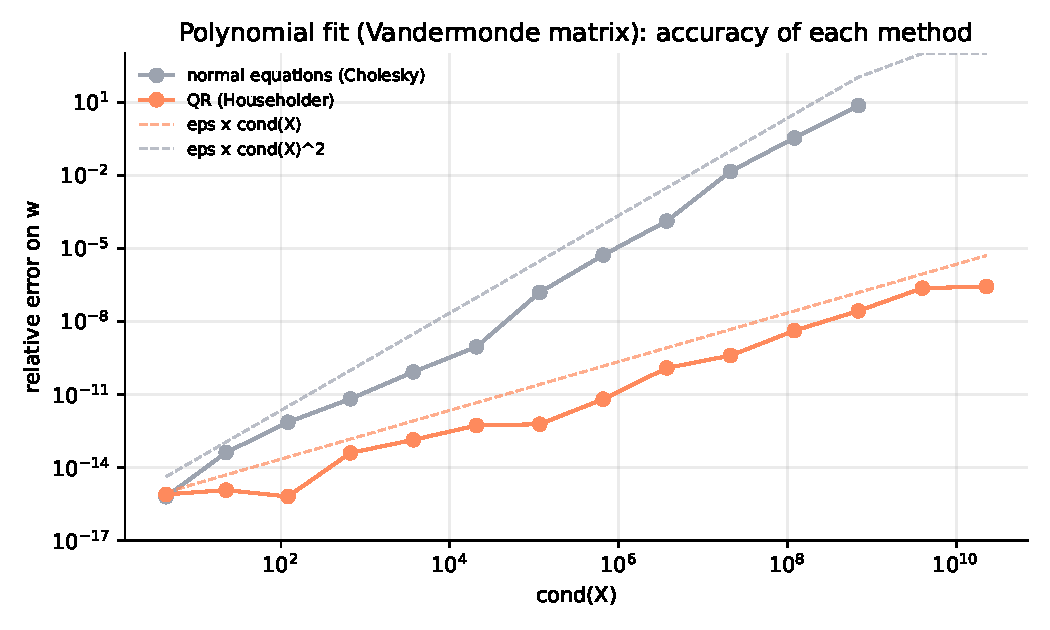
\includegraphics[width=0.72\textwidth]{../figures/4_stability.pdf}
\caption{L'erreur des équations normales suit $\varepsilon \cond(V)^2$, celle de QR suit $\varepsilon \cond(V)$. Au degré 14, $V^\top V$ n'est même plus numériquement définie positive et la factorisation de Cholesky échoue.}
\end{figure}

\section{Descente de gradient}

\subsection{Convergence et choix du pas}

La descente de gradient à pas fixe $\eta > 0$ s'écrit $w_{k+1} = w_k - \eta \nabla f(w_k)$. On note $0 < \mu = \lambda_{\min}(H) \le L = \lambda_{\max}(H)$ et $\kappa = L/\mu$ le conditionnement de $H$.

\begin{theoreme}
Soit $e_k = w_k - w^\star$ et $\rho(\eta) = \max\big(|1-\eta\mu|,\, |1-\eta L|\big)$. Alors
\[
  \lVert e_k \rVert_2 \le \rho(\eta)^k \lVert e_0\rVert_2 .
\]
La méthode converge pour tout point de départ si et seulement si $0 < \eta < 2/L$. Le pas optimal est $\eta^\star = \dfrac{2}{L+\mu}$, qui donne $\rho^\star = \dfrac{\kappa - 1}{\kappa + 1}$.
\end{theoreme}

\begin{proof}
Comme $\nabla f(w^\star) = 0$ et que $f$ est quadratique, $\nabla f(w_k) = H e_k$, donc $e_{k+1} = (I - \eta H)\, e_k$. La matrice $H$ est symétrique : dans une base orthonormée de vecteurs propres, $I - \eta H$ est diagonale, de coefficients $1 - \eta\lambda_i$ avec $\lambda_i \in [\mu, L]$. Sa norme $2$ vaut $\max_i |1-\eta\lambda_i| = \rho(\eta)$ (la fonction $\lambda \mapsto |1-\eta\lambda|$ étant convexe, son maximum sur $[\mu, L]$ est atteint aux bornes), d'où l'inégalité. Si $\eta > 2/L$, la composante de $e_0$ selon le vecteur propre associé à $L$ est multipliée par $|1-\eta L| > 1$ à chaque itération : elle diverge. Enfin, $\rho(\eta)$ est minimal quand $1-\eta\mu = -(1-\eta L)$, soit $\eta = 2/(L+\mu)$, et alors $\rho = \frac{L-\mu}{L+\mu} = \frac{\kappa-1}{\kappa+1}$.
\end{proof}

\begin{remarque}
Comme $f(w_k) - f(w^\star) = \frac12\, e_k^\top H e_k$, l'écart en valeur de la fonction décroît comme $\rho^{2k}$. C'est cette quantité que l'on mesure ci-dessous. Lorsque $L$ et $\mu$ sont inconnus, on peut choisir le pas à chaque itération par \emph{rebroussement d'Armijo} : on part de $t = 1$ et on divise $t$ par deux tant que $f(w - t\nabla f) > f(w) - \frac t2 \lVert\nabla f\rVert^2$. Cette variante est implémentée et testée.
\end{remarque}

\subsection{Vérification expérimentale}

Sur les données \emph{California Housing} standardisées (section~\ref{sec:california}), on obtient $\mu = \muH$, $L = \LH$, donc $\kappa = \kappaH$. Le taux observé est la pente de $\frac12 \log\big(f(w_k)-f^\star\big)$ en fonction de $k$.

\begin{table}[H]
\centering
\begin{tabular}{lccc}
\toprule
Pas $\eta$ & Taux théorique $\rho(\eta)$ & Taux observé & Itérations pour $f - f^\star < 10^{-10}$ \\
\midrule
\tableSteps
\bottomrule
\end{tabular}
\caption{Le taux mesuré coïncide avec la théorie à quelques millièmes près (pour le plus petit pas, la phase transitoire initiale accélère légèrement la décroissance) ; au-delà de $2/L$, la méthode diverge.}
\end{table}

\begin{figure}[H]
\centering
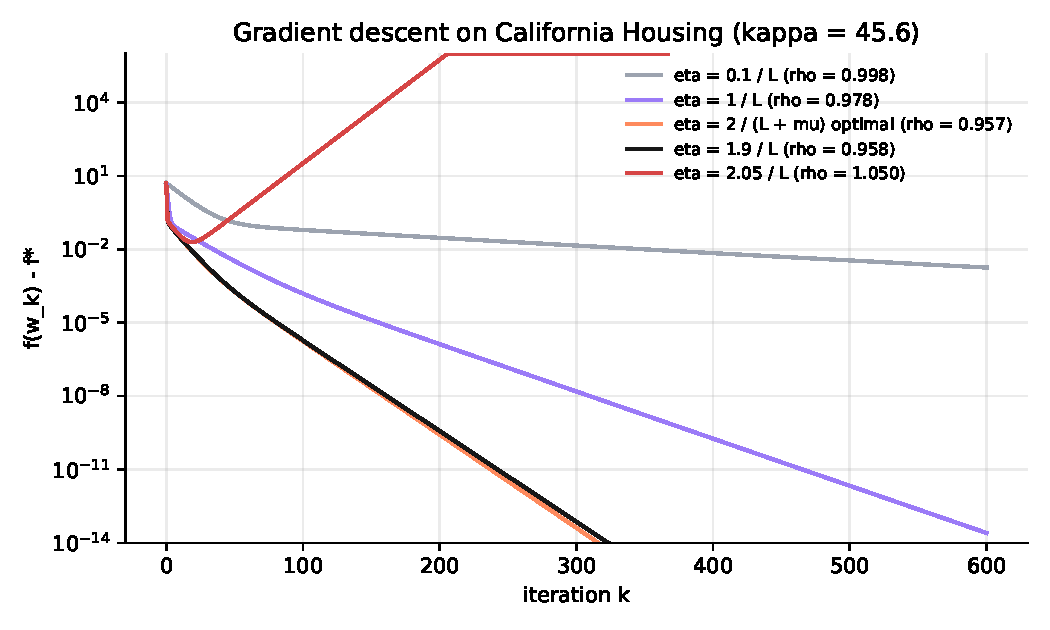
\includegraphics[width=0.75\textwidth]{../figures/2_step_sizes.pdf}
\caption{Décroissance de $f(w_k) - f^\star$ selon le pas. Le pas optimal $\eta^\star$ et le pas $1{,}9/L$ ont presque le même taux, car tous deux sont limités par la plus petite valeur propre $\mu$.}
\end{figure}

\subsection{Importance de la standardisation}

Le nombre d'itérations nécessaires est de l'ordre de $\kappa \log(1/\varepsilon)$. Sans standardisation, les variables ont des échelles très différentes (la population d'un îlot vaut plusieurs milliers, le revenu médian quelques unités) et $\kappa = \kappaRaw$ : après 2\,000 itérations au pas optimal, l'écart relatif $\frac{f(w_k)-f^\star}{f(w_0)-f^\star}$ vaut encore $\gapRaw$. Après standardisation, $\kappa = \kappaH$ et il descend à $\gapStd$ en moins de 400 itérations.

\begin{figure}[H]
\centering
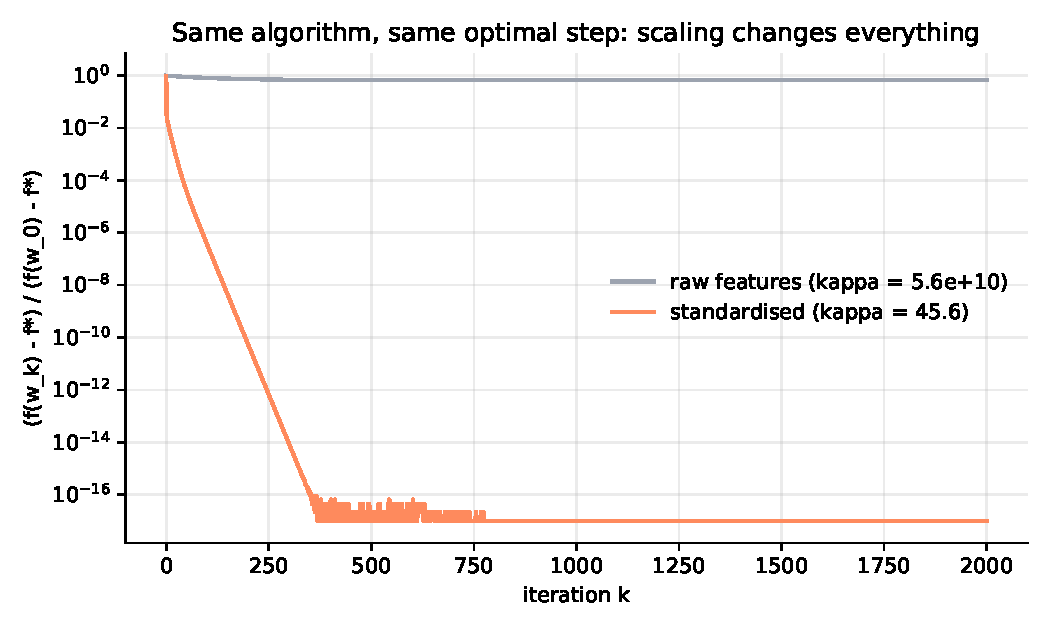
\includegraphics[width=0.72\textwidth]{../figures/3_scaling.pdf}
\caption{Même algorithme, même règle de pas : seule la mise à l'échelle des variables change.}
\end{figure}

\section{Application : le jeu de données California Housing}\label{sec:california}

\subsection{Données et préparation}

Chaque observation est un îlot du recensement californien de 1990. La variable à prédire est la valeur médiane des logements (en centaines de milliers de dollars), à partir de huit variables : revenu médian (\texttt{MedInc}), âge médian des logements (\texttt{HouseAge}), nombres moyens de pièces et de chambres par foyer (\texttt{AveRooms}, \texttt{AveBedrms}), population (\texttt{Population}), occupation moyenne (\texttt{AveOccup}), latitude et longitude. Les données proviennent de R.~K.~Pace et R.~Barry, \emph{Sparse spatial autoregressions}, Statistics \& Probability Letters, 1997. Les 207 lignes où le nombre de chambres manque sont retirées, ce qui laisse \nRows{} observations, séparées aléatoirement en \nTrain{} pour l'apprentissage et \nTest{} pour le test. La moyenne et l'écart-type de standardisation sont calculés sur l'échantillon d'apprentissage seulement.

\subsection{Résultats et comparaison avec scikit-learn}

\begin{table}[H]
\centering
\begin{tabular}{lcccc}
\toprule
Méthode & RMSE test (\$) & MAE test (\$) & $R^2$ test & $\max |w - w_{\text{sklearn}}|$ \\
\midrule
\tableMethods
\bottomrule
\end{tabular}
\caption{Les trois méthodes programmées retrouvent la solution de \texttt{scikit-learn} (\texttt{LinearRegression}). La descente de gradient au pas optimal converge en \gdIters{} itérations (norme du gradient $< 10^{-10}$).}
\end{table}

\begin{table}[H]
\centering
\begin{tabular}{lcc}
\toprule
Variable & Coefficient (QR) & \texttt{scikit-learn} \\
\midrule
\tableCoefs
\bottomrule
\end{tabular}
\caption{Coefficients du modèle sur variables standardisées : chacun mesure l'effet d'une augmentation d'un écart-type de la variable.}
\end{table}

Le revenu médian est la variable la plus influente : un écart-type de plus correspond à environ 82\,000~\$ de valeur médiane supplémentaire, toutes choses égales par ailleurs. La latitude et la longitude ont de forts coefficients négatifs : elles capturent la géographie (les prix sont plus élevés près de la côte et dans la baie de San Francisco ou autour de Los Angeles). Les signes opposés de \texttt{AveRooms} et \texttt{AveBedrms} s'expliquent par leur forte corrélation : à nombre de chambres fixé, davantage de pièces signifie des logements plus grands, mais les deux coefficients ne s'interprètent pas séparément.

\begin{figure}[H]
\centering
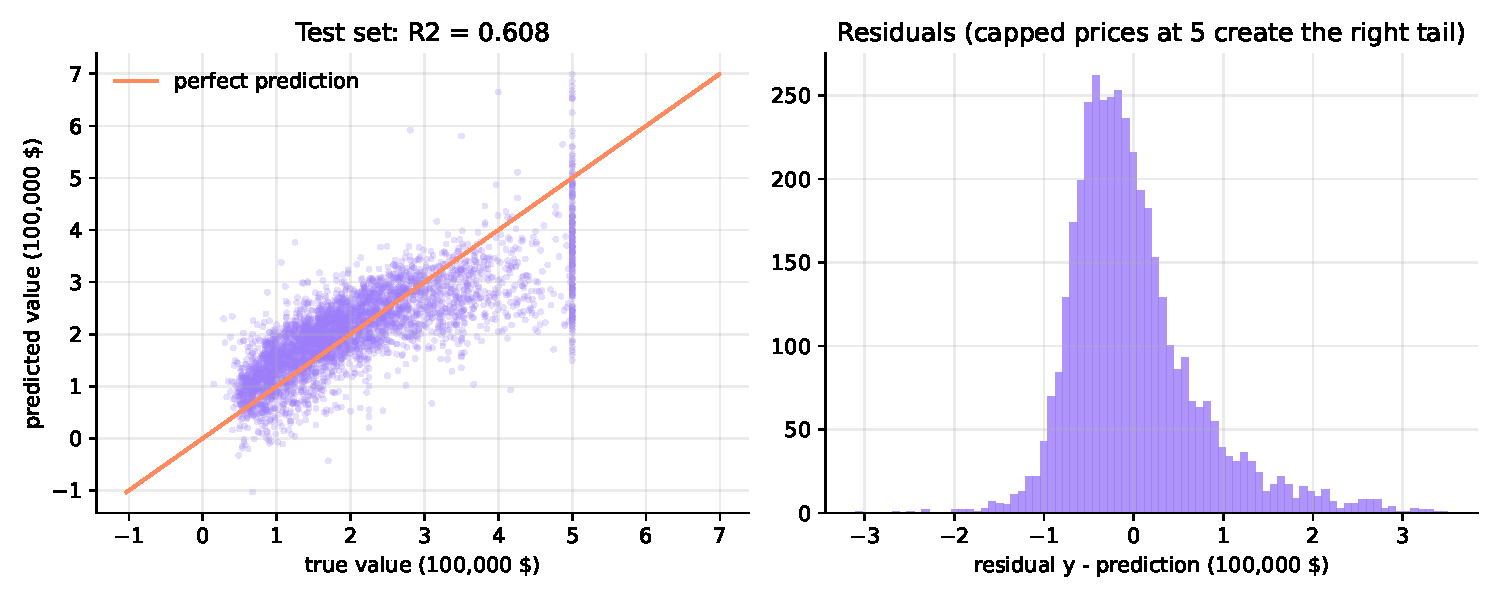
\includegraphics[width=0.95\textwidth]{../figures/1_predictions.pdf}
\caption{Prédictions sur l'échantillon de test. La colonne verticale à 5 vient des prix plafonnés à 500\,000~\$ dans les données d'origine.}
\end{figure}

\subsection{Limites du modèle}

Avec $R^2 = \rTwoQR$, le modèle linéaire explique environ 61\,\% de la variance. Ses limites sont visibles : la relation entre prix et localisation n'est pas linéaire, les prix plafonnés biaisent les grandes valeurs, et les résidus ont une queue à droite. Un modèle non linéaire ou des variables construites (distance à la côte, interactions) amélioreraient la prédiction ; l'objectif ici était d'étudier les méthodes de résolution, pas de maximiser le score.

\section{Conclusion}

Les trois méthodes, programmées à partir des seules opérations matricielles de NumPy, donnent la même solution que \texttt{scikit-learn} sur un jeu de données réel. Les expériences illustrent deux résultats d'analyse numérique : la méthode QR est préférable aux équations normales car son erreur dépend de $\cond(X)$ et non de $\cond(X)^2$, et la vitesse de la descente de gradient est gouvernée par le conditionnement $\kappa$ de la hessienne, que l'on améliore radicalement en standardisant les variables. Prolongements naturels : la régularisation de Tikhonov (ridge), qui remplace $X^\top X$ par $X^\top X + \lambda I$ et améliore le conditionnement ; la descente de gradient stochastique ; les méthodes de gradient accéléré (Nesterov), dont le taux dépend de $\sqrt\kappa$.

\appendix
\section{Reproduire les résultats}

Le code, les tests et ce rapport sont disponibles sur GitHub. Toutes les valeurs numériques de ce document sont générées automatiquement :
\begin{verbatim}
pip install -r requirements.txt
python experiments/run_all.py     # figures, results.md et report/generated.tex
pytest                            # 13 tests
cd report && pdflatex rapport.tex
\end{verbatim}

\end{document}
